\section{Part I: Analysis of Event Displays}
The first part of the analysis of data consists of looking at event displays, which are generated using \textit{GRope}. The main objective of this part is to understand how different channels affect different observed quantities and how we can come up with a filter to the quantities, so as to separate out different channels in a real world data. The filters are known as the cut criteria for this process. Every event display consists of an image and a list of quantities,
\begin{itemize}
    \item Ctrk(N): Number of charged tracks
    \item Ctrk(Sump): Momentum of all charged tracks
    \item Ecal(SumE): Total energy in the electromagnetic calorimeter
    \item Hcal(sumE): Total energy in the hadronic calorimeter
\end{itemize}
We have eight different samples for this part - four \textit{pure} samples and four \textit{mixed} samples. Each of the four \textit{pure} samples consists of only the events from a single channel, whereas the four \textit{mixed} samples consists of events from all the channels. We would analyse \textit{pure} samples first and come up with a cut criteria and test it on the \textit{mixed} samples and see how it fares.

\subsection{Analysis of $e^-e^+$-channel Samples}
The decay of $Z^0$ boson into an electron-positron pair is one of the channels of this process. For this case, we expect to detect two charged tracks. Since the pair has negligible mass compared to $Z^0$ boson, they carry away the center of mass energy, which implies \textit{SumP} will have this value. By construction of the detectors, we expect all the energy to be deposited in the electromagnetic calorimeter, while the signals should be close to zero in other components. The event display of a typical event can be found in \ref{fig:part1ee}, which shows two clear charged tracks and also shows that they deposit their energy in the electromagnetic calorimeter. By conservation of four-momenta, we should also expect to see the tracks exactly opposite to each other, which can also be seen here.

\subsection{Analysis of $\mu^-\mu^+$-channel Samples}
The decay of $Z^0$ boson into an muon-antimuon pair is another channel of this process. Just like the previous case, we expect to see two charged tracks and \textit{SumP} value being close to the center of mass energy value. By construction of the detectors, we expect close to zero energy deposit in the calorimeters. But instead, we expect to see a signal in the muon chambers. The event display of a typical event can be found in \ref{fig:part1mm}, which shows two clear charged charged tracks and signals in the muon chamber. We also see that conservation of four-momenta holds, since the tracks are exactly opposite to one another.

\subsection{Analysis of $\tau^-\tau^+$-channel Samples}
The decay of $Z^0$ boson into an tau-antitau pair is another channel of this process. Unlike its other leptonic cousins, $\tau$ has a much shorter life, which results in interesting outcomes here. We expect to see a large number of charged tracks due to the decay, clustered exactly opposite to each other due to conservation of four-momenta. The dominant decay products are $\mu$ and $\pi$, which can then be detected in the other components of the detectors. This channel can be classified by the number of charge tracks, called \textit{prongs}. The event display of a \textit{3-prong} event can be found in \ref{fig:part1tt}. We can see the signals in muon chamber on one side and we can also see the deposit in electromagnetic calorimeter and hadronic calorimeter on the other side, which corresponds to the pions. We should also expect the \textit{SumP} value to be less than the center of mass energy, since neutrinos are produced to conserve lepton number, which carry away some of the energy. Unlike the previous two cases, this channel doesn't have a very distinct filter property at the first sight.

\subsection{Analysis of $q\bar{q}$-channel Samples}
The decay of $Z^0$ boson into an quark-antiquark pair is another channel of this process. Since quarks cannot exist as free particles, they produce hadrons, which then decay into further particles that can be then detected at various components. This results in the so-called \textit{jets}, which are much bigger clusters of charged tracks. Depending on the final products, we expect to notice signals in all of the components of the detectors. But one distinct property of this channel is the large number of charged tracks produced. The event display of a typical event can be found in \ref{fig:part1qq}, which clearly shows the jets. Again, we expect the \textit{SumP} value to be lesser than center of mass energy, since depending on the decay products, various neutrinos are produced to conserve lepton number, which carry away some of the energy.

\subsection{Developing the cuts}
With this, we now first extract the information of how different quantities behave for the different \textit{pure} samples. The raw data can be found in the appendix \ref{table:ed-ee}, \ref{table:ed-mm}, \ref{table:ed-tt} and \ref{table:ed-qq}. We plot histograms of all these quantities for different channels and identify \textit{cuts} on the quantities to separate out the channels. The histograms are given in the fig \ref{fig:hist}. The bin sizes are chosen so that we are able to see the best possible separation of the different channels.\\
\begin{figure}[h!]
    \centering
    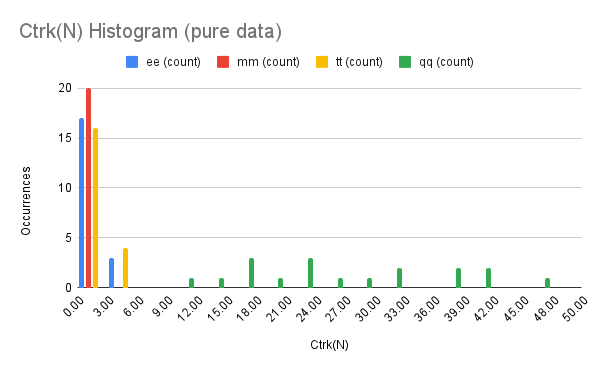
\includegraphics[width = 0.45\textwidth]{CtrkN-pure.png}
    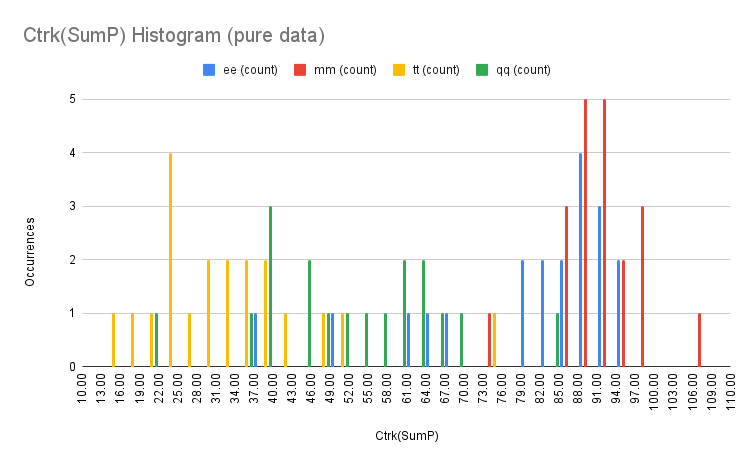
\includegraphics[width = 0.45\textwidth]{CtrkP-pure.png}
    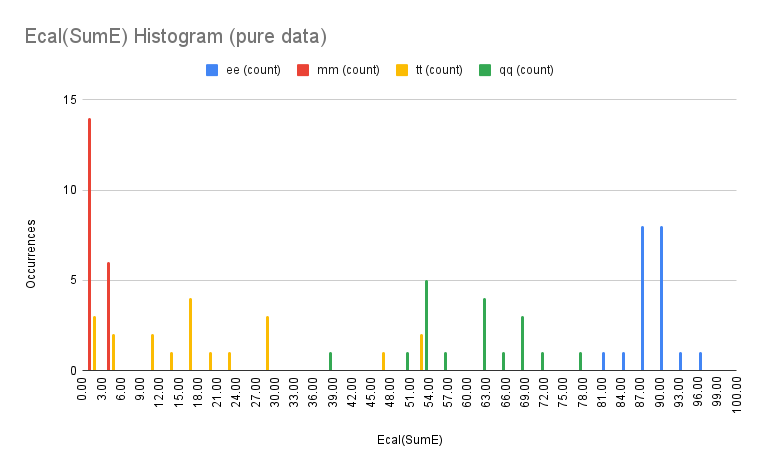
\includegraphics[width = 0.45\textwidth]{Ecal-pure.png}
    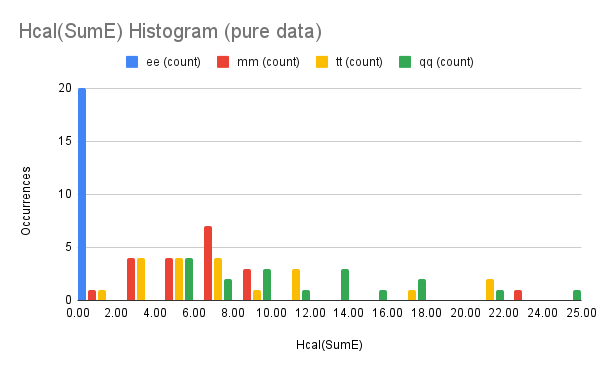
\includegraphics[width = 0.45\textwidth]{Hcal-pure.png}
    \caption{Histograms of \textit{Ctrk(N)}, \textit{Ctrk(Sump)}, \textit{Ecal(SumE)} and \textit{Hcal(SumE)} for the four channels, generated from \textit{pure} samples.}
    \label{fig:hist}
\end{figure}
We see that \textit{Ctrk(N)} clearly lets us distinguish $q\bar{q}$ channel events from the other channels. Therefore, we require the value of \textit{Ctrk(N)} to be greater than or equal to $8$ to seperate the hadronic channel and we require the value of \textit{Ctrk(N)} to be lesser than $6$ to separate all the leptonic channels. Note that this cut alone completely separates the hadronic channel events from the leptonic channel events. We see from the histogram for \textit{Ctrk(Sump)} that we can separate muon channel and tau channel from each other by requiring \textit{Ctrk(Sump)} greater than or equal to $75$ for muon channel and lesser than or equal to $75$ for tau channel. We do not impose cuts on any other channel for this quantity. Note that this separates only the muon and tau channel from each other, but these two events may still contain electron and hadronic channel events. This cut, when used with all the other cuts, ensures that we completely separate the channels from one another. We see from the histogram for \textit{Ecal(SumE)} that it is possible to completely distinguish electron and muon events. This was expected from what we discussed previously. We require the value of \textit{Ecal(SumE)} greater than or equal to $80$ for electron channel and lesser than or equal to 10 for muon channel. We also impose a minor cut for tau channel - \textit{Ecal(SumE)} less than or equal to 60 and for hadronic channel - \textit{Ecal(SumE)} lies between $36$ and $79$. We see from the histogram for \textit{Hcal(SumE)} that it is possible to completely separate electron channel from the other channel by requiring \textit{Hcal(SumE)} to be less than $1$. This quantity does not give us any other cut to separate out other channels. The final cuts are given in the table \ref{table:cuts}.\\
\begin{table}[h!]
\centering
\begin{tabular}{c|cccc}
\hline
Channel        & Ctrk(N)          & Ctrk(Sump)        & Ecal(SumE)        & Hcal(SumE)   \\
\hline
$e^-e^+$       & (0,6)            &                   & \textgreater{}=80 & \textless{}1 \\
$\mu^-\mu^+$   & \textless{}6     & \textgreater{}=75 & \textless{}=10    &              \\
$\tau^-\tau^+$ & \textless{}6     & \textless{}=75    & \textless{}=60    &              \\
$q\bar{q}$     & \textgreater{}=8 &                   & {[}36,79{]}       &             \\ \hline
\end{tabular}
\caption{Cuts determined from event display analysis}
\label{table:cuts}
\end{table}
We now test the determined cuts on \textit{mixed} samples. The raw data and the channel determined using the cuts can be found in \ref{table:ed-mixed}. The event display was then checked visually if it matched the channel as determined by the cuts. We found that the all the events were determined accurately with our cuts. But we are not sure how perfect our cuts will be, when tested against real world data. For this purpose, we would like to refine our cuts before we carry out a statistical analysis. This is done in the first part of the next section.

\section{Part II: Statistical Analysis of $Z^0$ Decays}
In the previous subsection, we carried out an analysis based on event displays. This was possible because we did not have a lot of events to work with. Obviously, such an analysis would prove to be futile if we try to carry it out on a large set of data. Analysis of large sets of data would be the primary discussion of this subsection. We use the software, $ROOT$ to analyse the data on a statistical basis. \textit{ROOT} works with \textit{.root} files, which contain all the information in a tree-like structure, called \textit{ntuple}. The contents of the \textit{ntuple} are,
\begin{itemize}
    \item RUN: Run number
    \item EVENT: Event number
    \item NCHARGED: Number of charged tracks
    \item PCHARGED: Total scalar sum of track momenta
    \item E\_ECAL: Total energy in electromagnetic calorimeter
    \item E\_HCAL: Total energy in hadronic calorimeter
    \item E\_LEP: LEP beam energy ($=\sqrt{s}/2$)
    \item COS\_THRU: cos(polar angle) between beam axis and thrust axis
    \item COS\_THET: cos(polar angle) between incoming positron and outgoing positive particle
\end{itemize}
We also have two categories of data, each containing a lot of \textit{ntuples},
\begin{itemize}
    \item Monte Carlo (MC): These correspond to the ``\textit{pure}'' events from the previous subsection. These are simulated - detector response to a calculated outgoing momentum four-vector for a specific process.
    \item Data: These correspond to the ``\textit{mixed}'' events from the previous subsection. These are real life data recorded with the OPAL detector at specific energies around the $Z^0$ resonance maximum.
\end{itemize}
\textit{ROOT} can be used to set cuts on the above variables in a data and get histograms of different variables. This allows for a statistical analysis of the data. All the above information can be found in \cite{UB}.

\subsection{Refining the cuts}
As mentioned previously, we have two categories of data. There are four Monte Carlo (MC) data, one for each of the decay channels. There are six real world data and we will be using \textit{data6.root} for our analysis in the following parts. Analysis of event displays already gave us an idea of what cuts to use, to extract the different channels. Our first step here will be to test our cuts on the MC data and check how they fare. And the second step will be to refine the cuts a little so that we are better able to extract different channels.\\
When it comes to $e^-e^+$ final state decay channel, we would like to exclude t-channel events. This is because t-channel is possible only in the mode and for the sake of consistency, we would like to limit ourselves to only s-channel. From theory\cite{UB}, we know that the t-channel dominates at large $cos\theta$. By introducing a new cut to exclude events with large $cos\theta$, we eliminate a most of the t-channel events. But this also means that we are eliminating some of the s-channel events. To account for this, we multiply the observed events after applying the modified cuts with correction factor. This correction factor is given by,
\begin{equation}
    \delta = \frac{\int_{-1}^1 (1 + x^2) dx}{\int_{-0.9}^{0.5} (1 + x^2) dx} \approx 1.5829.
\end{equation}
This factor is arrived at from theory, which gives the behaviour of s-channel as proportional to $(1 + cos^2\theta)$ and the integral limits are correspond to the $cos\theta$ values which we exclude.\\
When it comes to $\mu^-\mu^+$ final state decay channel, we observed a lot of events with \textit{PCHARGED} equal to exactly $0$. These events are not physical. Hence we apply a cut to eliminate such events. In the cases of $e^-e^+$ and $\mu^-\mu^+$, we also exclude $cos\theta$ values very close to $1$ and $-1$, as the detector resolution is far from perfect close to the beam axis. To summarise, we have the following additions - $cos\theta \in [-0.9, 0.5]$, to remove t-channel events in the case of $e^-e^+$, $PCHARGED > 0$, to exclude unphysical events in the case of $e^-e^+$ and $cos\theta \in [-0.9, 0.9]$, to eliminate low resolution events in the cases of $e^-e^+$ and $\mu^-\mu^+$. Interestingly, the channels $\tau^-\tau^+$ and $q\bar{q}$ did not require any additional global cuts. But, we did add the cut $cos\theta \in [-1, 1]$ to remove any unphysical events. Analysis done with \textit{ROOT} on the $e^-e^+$ MC can be found in the appendix, \ref{fig:global-ee}, \ref{fig:eecutee}, \ref{fig:mmcutee}, \ref{fig:ttcutee} and \ref{fig:qqcutee}. Analysis on the other MC files and ultimately the data file are done similarly.\\
After testing our cuts, we arrive at the conclusion that we don't need any further refinements other than the additions mentioned above. With these additions, we go about analysing \textit{data6.root}. The raw data of observed events using our cuts is given in the table \ref{table:eventsdata6} below. Note that the correction factor has not been applied to the $e^-e^+$ event numbers but it is used in our latter calculations. The event numbers are exactly what we get after applying all the cuts appropriately.

\begin{table}[!h]
\centering
\resizebox{\columnwidth}{!}{
\begin{tabular}{cccccc}
\hline
\multicolumn{1}{|c|}{}               & \multicolumn{5}{c|}{Number of observed events}                                                                                                                                                                                                                    \\ \hline
\multicolumn{1}{|c|}{MC Sample}      & \multicolumn{1}{c|}{$e^-e^+$ cuts} & \multicolumn{1}{c|}{$\mu^-\mu^+$ cuts} & \multicolumn{1}{c|}{$\tau^-\tau^+$ cuts} & \multicolumn{1}{c|}{$q\bar{q}$ cuts} & \multicolumn{1}{c|}{\begin{tabular}[c]{@{}c@{}}Total \\ (incl. global cuts, if any)\end{tabular}} \\ \hline
\multicolumn{1}{|c|}{$e^-e^+$}       & \multicolumn{1}{c|}{18835}         & \multicolumn{1}{c|}{0}                 & \multicolumn{1}{c|}{378}                 & \multicolumn{1}{c|}{0}               & \multicolumn{1}{c|}{56720}                                                                        \\
\multicolumn{1}{|c|}{$\mu^-\mu^+$}   & \multicolumn{1}{c|}{0}             & \multicolumn{1}{c|}{76209}             & \multicolumn{1}{c|}{8599}                & \multicolumn{1}{c|}{0}               & \multicolumn{1}{c|}{89887}                                                                        \\
\multicolumn{1}{|c|}{$\tau^-\tau^+$} & \multicolumn{1}{c|}{26}            & \multicolumn{1}{c|}{35}                & \multicolumn{1}{c|}{71131}               & \multicolumn{1}{c|}{135}             & \multicolumn{1}{c|}{79214}                                                                        \\
\multicolumn{1}{|c|}{$q\bar{q}$}    & \multicolumn{1}{c|}{0}            & \multicolumn{1}{c|}{0}                & \multicolumn{1}{c|}{173}                  & \multicolumn{1}{c|}{92164}            & \multicolumn{1}{c|}{98563}                                                                                             \\ \hline
\end{tabular}
}
\caption{Number of events with different cuts applied to each of the MC data.}
\label{table:eventsdata6}
\end{table}

\subsection{Efficiency Matrix}
The efficiency matrix is a measure of how efficient the cuts are at extracting the different decay channels. If we consider the actual event numbers of the different channels as a $4 \times 1$ matrix, the efficiency matrix will be a $4 \times 4$ matrix and ideally, it should be a unit matrix. In this case, the event numbers observed matches the actual event numbers. But this is not the case usually. We should aim to achieve an efficiency matrix with diagonal elements as close to $1$ as possible and the off-diagonal elements as close to $0$ as possible. The efficiency matrix elements are given by\cite{UB},
\begin{equation}
    \epsilon_{ij} = \frac{N^{i, cut}_j}{N^{j, all}_j}.
\end{equation}
For example, $\epsilon_{12}$ corresponds to $e^-e^+$ cuts applied to $\mu^-\mu^+$ events divided by the total observed $\mu^-\mu^+$ events. Note that we construct the $4 \times 1$ matrix in the following order - $e^-e^+$ events, $\mu^-\mu^+$ events, $\tau^-\tau+$ events and $q\bar{q}$ events. With this efficiency matrix, one could extract the actual event numbers as follows,
\begin{equation}
    N_{obs} = \epsilon N_{actual} \implies N_{actual} = \epsilon^{-1} N_{obs}.
\end{equation}
This gives us an efficiency matrix,
\begin{equation}
    \epsilon = 
    \begin{pmatrix}
        5.26 \times 10^{-1} & 0 & 3.28 \times 10^{-4} & 0 \\
        0 & 8.48 \times 10^{-1} & 4.42 \times 10^{-4} & 0 \\
        6.66 \times 10^{-3} & 9.57 \times 10^{-2} & 8.98 \times 10^{-1} & 1.76 \times 10^{-3} \\
        0 & 0 & 1.70 \times 10^{-3} & 9.35 \times 10^{-1}
    \end{pmatrix}.
\end{equation}
Given a cut, whether or not a particular event passes it can be modelled with a binomial distribution, just like modelling a coin toss. In the limit when such an ``experiment'' is conducted on large sample size, the probability mass function of the binomial distribution can be approximated by a normal distribution. In which case, the standard deviation is given by,
\begin{equation}
    \Delta \epsilon_{ij} = \sqrt{\frac{\epsilon_{ij}(1-\epsilon_{ij})}{N}},
\end{equation}
where $\epsilon_{ij}$ is a particular element of the efficiency matrix and $N$ is the total events corresponding to that matrix element. The above treatment can be found in any introductory book on probability theory, for example Feller\cite{feller}. This gives us the standard deviation in the efficiency matrix elements,
\begin{equation}
    \Delta \epsilon = 
    \begin{pmatrix}
        2.10 \times 10^{-3} & 0 & 6.44 \times 10^{-5} & 0 \\
        0 & 1.12 \times 10^{-3} & 7.47 \times 10^{-5} & 0 \\
        3.41 \times 10^{-4} & 9.81 \times 10^{-4} & 1.08 \times 10^{-3} & 1.33 \times 10^{-4} \\
        0 & 0 & 1.46 \times 10^{-4} & 7.85 \times 10^{-5}
    \end{pmatrix}.
\end{equation}
For our calculations in the following sections, we require $N_{actual}$. Therefore, we invert the matrix. The calculations for error in the inverse matrix elements is not straightforward. We refer to \cite{lefebvre}, which gives the error in the inverse matrix element to be,
\begin{equation}
    (\Delta \epsilon^{-1})^2_{ij} = \sum_{\alpha = 1}^4 \sum_{\beta = 1}^4 (\epsilon^{-1})^2_{i\alpha}(\Delta \epsilon)^2_{\alpha\beta} (\epsilon^{-1})^2_{\beta j}.
\end{equation}
With this we get the following inverse efficiency matrix and the error in the inverse efficiency matrix elements,
\begin{equation}
\begin{split}
    \epsilon^{-1} = 
    \begin{pmatrix}
        1.90 & 7.85 \times 10^{-5} & -6.95 \times 10^{-4} & 1.30 \times 10^{-6} \\
        7.36 \times 10^{-6} & 1.18 & -5.80 \times 10^{-4} & 1.09 \times 10^{-6} \\
        -1.41 \times 10^{-2} & -1.26 \times 10^{-1} & 1.11 & -2.09 \times 10^{-3} \\
        2.57 \times 10^{-5} & 2.29 \times 10^{-4} & -2.03 \times 10^{-3} & 1.07
    \end{pmatrix}
    \pm \\
    \begin{pmatrix}
        7.59 \times 10^{-3} & 1.54 \times 10^{-5} & 1.36 \times 10^{-4} & 2.75 \times 10^{-7} \\
        1.30 \times 10^{-6} & 1.67 \times 10^{-3} & 9.81 \times 10^{-5} & 2.02 \times 10^{-7} \\
        7.26 \times 10^{-4} & 1.31 \times 10^{-3} & 1.33 \times 10^{-3} & 1.59 \times 10^{-4} \\
        2.58 \times 10^{-6} & 1.98 \times 10^{-5} & 1.75 \times 10^{-4} & 8.98 \times 10^{-4}
    \end{pmatrix}
\end{split}
\end{equation}

\subsection{Cross Sections}
With the above inverse efficiency matrix, we can now calculate the actual event numbers and hence, the cross sections corresponding to different modes. The actual event numbers, $N_{actual}$, will simply be $\epsilon^{-1} N_{obs}$, as explained earlier. The error in actual event numbers is then,
\begin{equation}
    \Delta N_{obs, i} = \sqrt{\sum_{j=1}^4 N_{obs, j}^2 (\Delta \epsilon_{ij}^{-1})^2 + 
    \sum_{j=1}^4 (\epsilon_{ij}^{-1})^{2} N_{obs, j}}.
\end{equation}
The events are assumed to obey Poisson statistics and hence, $\Delta N_{obs}$ is taken as $\sqrt{N_obs}$. With the actual event numbers, we can calculate the cross section as,
\begin{equation}
    \sigma = \frac{N_{actual}}{\int \mathcal{L} dt} + \text{cf(radiation)},
\end{equation}
with the errors,
\begin{equation}
    \Delta \sigma = \sqrt{\frac{(\Delta N_{actual})^2}{(\int \mathcal{L} dt)^2} + 
    \frac{N_{actual}^2 (\Delta \int \mathcal{L} dt)^2}{(\int \mathcal{L} dt)^4}}.
\end{equation}
where $\int \mathcal{L} dt$ is the integrated luminosity and $\text{cf(radiation}$ is the radiative correction factors. We use the integrated luminosity values and the radiative correction factors from from \cite{UB}. The actual event numbers, integrated luminosity values and the radiative correction factor can be found in the tables \ref{table:actualnumbers}, \ref{table:intlum} in the appendix and the calculated cross sections for different $\sqrt{s}$ values can be found in the table \ref{table:cross-section}.
\begin{table}[!h]
\centering
\begin{tabular}{c|cccc}
\hline
$\sqrt{s}$ {[}GeV{]} & $\sigma_{ee}$ {[}nb{]} & $\sigma_{mm}$ {[}nb{]} & $\sigma_{tt}$ {[}nb{]} & $\sigma_{qq}$ {[}nb{]} \\
\hline
88.47                & 0.39 $\pm$ 0.03        & 0.30 $\pm$ 0.02        & 0.47 $\pm$ 0.03        & 7.19 $\pm$ 0.10        \\
89.46                & 0.82 $\pm$ 0.04        & 0.65 $\pm$ 0.03        & 0.72 $\pm$ 0.03        & 14.20 $\pm$ 0.14       \\
90.22                & 1.26 $\pm$ 0.04        & 1.16 $\pm$ 0.03        & 1.12 $\pm$ 0.03        & 25.70 $\pm$ 0.21       \\
91.22                & 1.69 $\pm$ 0.02        & 1.82 $\pm$ 0.02        & 1.75 $\pm$ 0.02        & 40.75 $\pm$ 0.22       \\
91.97                & 1.12 $\pm$ 0.05        & 1.32 $\pm$ 0.04        & 1.21 $\pm$ 0.04        & 28.96 $\pm$ 0.27       \\
92.96                & 0.45 $\pm$ 0.04        & 0.55 $\pm$ 0.03        & 0.66 $\pm$ 0.04        & 13.67 $\pm$ 0.20       \\
93.71                & 0.28 $\pm$ 0.03        & 0.34 $\pm$ 0.02        & 0.40 $\pm$ 0.03        & 8.20 $\pm$ 0.13       \\
\hline
\end{tabular}
\caption{Calculated cross section values for different $\sqrt{s}$ values.}
\label{table:cross-section}
\end{table}

\subsection{Forward Backward Asymmetry and Weak mixing angle}
As discussed earlier in Section \ref{FBasymm}, the forward-backward asymmetry arises as a result of the different couplings of the $Z^{0}$ to left handed and right handed fermions, and the weak mixing (Weinberg) angle can be extracted from this factor. We consider the $\mu^-\mu^+$ decay channel as we don't have the problem of t-channel like in the $e^-e^+$ decay mode. We also get two clear tracks in the case of $\mu^-\mu^+$ decay mode. We can calculate the asymmetry by measure the event numbers for $cos\theta > 0$ and $cos\theta < 0$. The forward backward asymmetry then is,
\begin{equation}
    A_{fb} = \frac{N_+ - N_-}{N_+ + N_-} + \text{cf($A_{fb}$)},
\end{equation}
where $N_+$ is the event numbers with $cos\theta > 0$ and $N_-$ is the event numbers with $cos\theta < 0$, cf($A_{fb}$) is the $A_{fb}$ correction factor, which can be found in the table \ref{table:intlum}. The error in $A_{fb}$ is given by,
\begin{equation}
    \Delta A_{fb} = \sqrt{N_-\left(\frac{2N_+}{(N_+ + N_-)^2}\right)^2 + 
    N_+\left(\frac{2N_-}{(N_+ + N_-)^2}\right)^2}.
\end{equation}
The calculated $A_{fb}$ can be found in table \ref{table:afb}.\\
\begin{table}[h!]
\centering
\begin{tabular}{c|ccc}
\hline
$\sqrt{s}$ {[}GeV{]} & $N_+$ & $N_-$ & $A_{fb}$           \\ \hline
                    & \multicolumn{3}{c}{$\mu^-\mu^+$ data}  \\ \hline
88.47                & 51    & 69    & -0.128 $\pm$ 0.090 \\
89.46                & 148   & 156   & -0.007 $\pm$ 0.057 \\
90.22                & 272   & 319   & -0.063 $\pm$ 0.041 \\
91.22                & 4297  & 4384  & 0.008 $\pm$ 0.011  \\
91.97                & 387   & 380   & 0.039 $\pm$ 0.036  \\
92.96                & 173   & 123   & 0.231 $\pm$ 0.057  \\
93.71                & 189   & 150   & 0.209 $\pm$ 0.054  \\ \hline
                     & \multicolumn{3}{c}{$\mu^-\mu^+$ MC}  \\ \hline
91.22                & 37807 & 38402 & 0.010 $\pm$ 0.014    \\ \hline
\end{tabular}
\caption{Forward and Backward event numbers for $\mu^-\mu^+$ mode data and MC events with the calculated $A_{fb}$ values.}
\label{table:afb}
\end{table}
With this, we can calculate the weak mixing angle. For the data events, we consider the $A_{fb}$ value at $Z^0$ resonance energy and calculate the weak mixing angle (using Eq. \ref{eqn:Weinbergangle}) as,
\begin{equation}
    sin^2\theta_W = 0.2369 \pm 0.0085,
\end{equation}
and for the MC event, we calculate the weak mixing angle as,
\begin{equation}
    sin^2\theta_W = 0.2352 \pm 0.0098.
\end{equation}
The literature value for weak-mixing angle is $sin^2\theta_W = 0.23122 \pm 0.00003$ \cite{pdg-ew}. This value is within one standard deviation of both the results calculated with the $\mu^-\mu^+$ MC and the data file.

\subsection{Lepton Universality}
Lepton universality states that, since the masses of leptons are much smaller compared to that of the $Z^0$ boson, the cross section of all the three leptonic decay modes must be the same, at $Z^0$ resonance. From the table \ref{table:cross-section}, we can see that at $Z^0$ resonance ($=91.22 GeV$),
\begin{equation}
\begin{split}
    \sigma_e = 1.69 \pm 0.02 ~ \text{nb} \\
    \sigma_{\mu} = 1.82 \pm 0.02 ~ \text{nb} \\
    \sigma_{\tau} = 1.75 \pm 0.02 ~ \text{nb}
\end{split}
\end{equation}
We see that even though the values are almost equal, they are not exactly equal. The theoretical value calculated with values from \cite{UB} gives $\sigma_f = 1.99 nb$. We see that the values calculated from the data are several standard deviations away from the theoretical value, even though they match up to the order and in fact, quite close. We postulate that this is due to the fact that we don't have the best possible cut criteria. That is, we are undercounting the event numbers to some extent, which results in the lower cross section values. And since the factor by which we undercount differs between different modes, we get cross sections that slightly differ from each other. This problem could be overcome by substantially increasing the number of events. We calculate the ratios of the hadronic to the leptonic modes as follow,
\begin{equation}
\begin{split}
    \frac{\sigma_{had}}{\sigma_e} = 24.18 \pm 0.30 \\
    \frac{\sigma_{had}}{\sigma_{\mu}} = 22.43 \pm 0.24 \\
    \frac{\sigma_{had}}{\sigma_{\tau}} = 23.28 \pm 0.26
\end{split}
\end{equation}
The ratios above directly reflect the deviations we had in the cross section values and a little greater than the theoretical value. The literature values are given by $\frac{\sigma_{had}}{\sigma_e} = 20.804 \pm 0.050$, $\frac{\sigma_{had}}{\sigma_{\mu}} = 20.785 \pm 0.033$ and $\frac{\sigma_{had}}{\sigma_{\tau}} = 20.764 \pm 0.045$ respectively \cite{pdg2}. Again, we are several orders of standard deviation away. But, both they are of the same order of magnitude and comparable. This means that the problem in our data is not fundamental and could be overcome by improving our counts.

\subsection{Breit-Wigner Fit of Cross Section}
Now we extract the all important quantities from our data. To do this, we fit our cross section values against a Breit-Wigner curve of the form,
\begin{equation}
    \sigma_f (s) = \frac{12\pi}{M_Z^2} \frac{s \Gamma_e \Gamma_f}{(s-M_Z^2)^2 + \left(\frac{s\Gamma_Z}{M_Z}\right)^2} (\hbar^2 c^2),
\end{equation}
which has three parameters, $M_Z$, $\Gamma_Z$ and $\Gamma_e\Gamma_f$. The factor $\hbar^2 c^2 = 3.893793719 \times 10^5 \text{nb GeV$^2$}$ is used to convert the cross section values to SI units from natural units. We used \textit{scipy.optimize} module for \textit{Python} to fit the function against our data. The plots are given in \ref{fig:bwfit}. The fit parameters obtained along with the reduced $\chi^2$ values for the fit can be found in the table \ref{table:bwfit}.\\
\begin{figure}[h!]
\begin{center}
    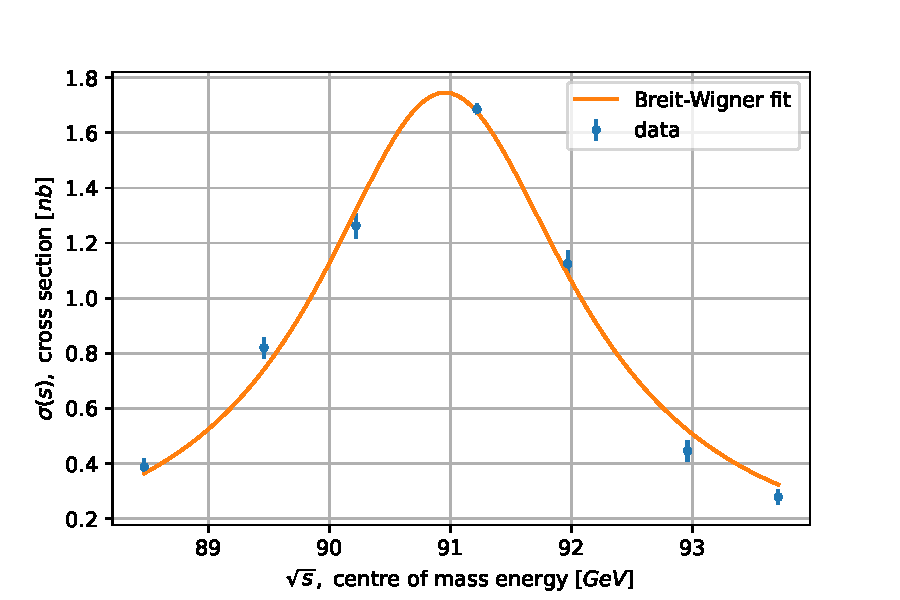
\includegraphics[width = 0.45\textwidth]{e213-ee-fit.pdf}
    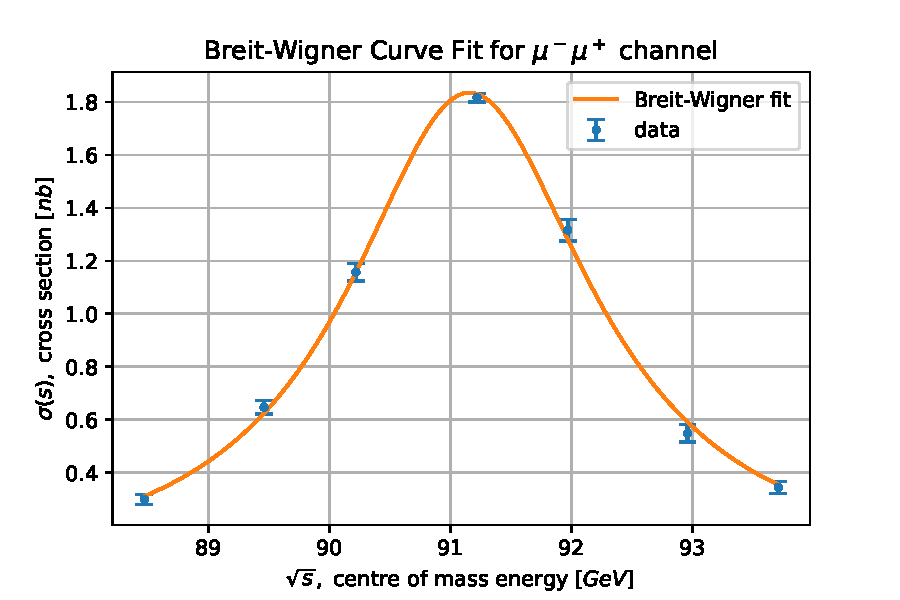
\includegraphics[width = 0.45\textwidth]{e213-mm-fit.pdf}
    
\includegraphics[width = 0.45\textwidth]{e213-tt-fit.pdf}
    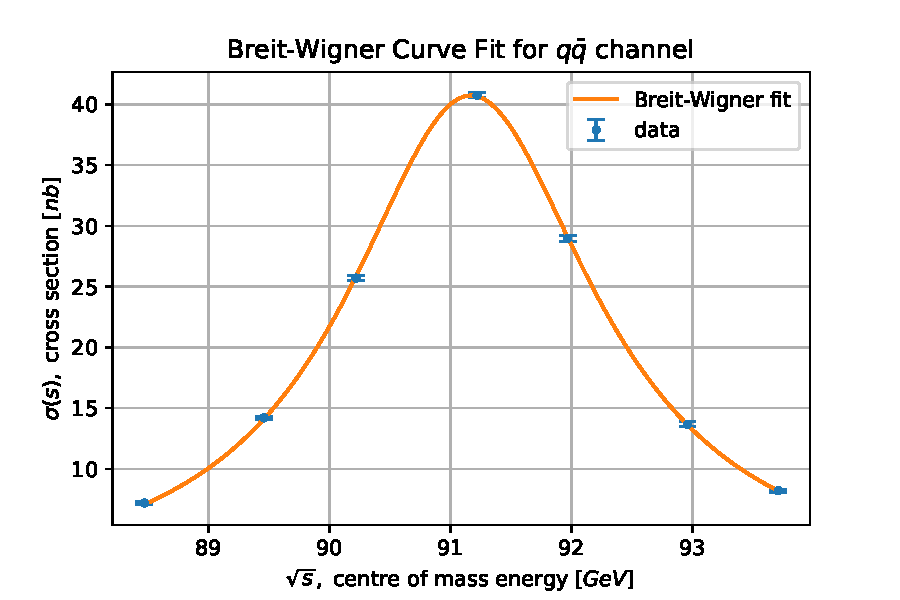
\includegraphics[width = 0.45\textwidth]{e213-qq-fit.pdf}
\end{center}
\caption{Breit-Wigner fits for the four different decay channels}
\label{fig:bwfit}
\end{figure}
\begin{table}[h!]
\centering
\begin{tabular}{c|cccc}
\hline
Channel        & $M_Z$ {[}GeV{]}    & $\Gamma_Z$ {[}GeV{]} & $\Gamma_e\Gamma_f$ {[}GeV$^2${]}                   & $\chi_{red}^2$ \\ \hline
$e^-e^+$       & 90.973 $\pm$ 0.047 & 2.591 $\pm$ 0.158    & 6.615$\times$10$^{-3}$ $\pm$ 6.29$\times$10$^{-4}$ & 3.47           \\
$\mu^-\mu^+$   & 91.117 $\pm$ 0.021 & 2.462 $\pm$ 0.060    & 6.306$\times$10$^{-3}$ $\pm$ 2.46$\times$10$^{-4}$ & 1.10           \\
$\tau^-\tau^+$ & 91.159 $\pm$ 0.058 & 2.825 $\pm$ 0.179    & 7.690$\times$10$^{-3}$ $\pm$ 7.85$\times$10$^{-4}$ & 8.34           \\
$q\bar{q}$     & 91.187 $\pm$ 0.004 & 2.515 $\pm$ 0.010    & 0.1460 $\pm$ 0.0009                                & 0.58          \\ \hline
\end{tabular}
\caption[Breit-Wigner fit parameters and reduced $\chi^2$ values for the data]{Fit parameters and reduced $\chi^2$ values for the data}
\label{table:bwfit}
\end{table}
We have three parameters and seven data points. This gives us $4$ degrees of freedom for our fit. The $\mu^-\mu^+$ fit gives the best reduced $\chi^2$ value. The reduced $\chi^2$ value for $q\bar{q}$ is less than 1, which implies that we are over-fitting the data or the error variances are overestimated. The reduced $\chi^2$ value for $e^-e^+$ is greater than 1, which implies that we are under-fitting the data or the error variances are underestimated. Whereas, the reduced $\chi^2$ value for $\tau^-\tau^+$ is much greater than 1, which implies that we don't have a good fit\cite{bevington}. But, none of the fits have a corresponding $p-valule$ less than $0.05$, which means they're not significant enough to be considered seriously different from previous literature results\cite{pvalue}. One major issue with using reduced $\chi^2$ statistic test here is that we have only a limited number of points. Therefore, we don't have a lot of freedom to fit the data with. This ultimately results in a bad value, even though the fit is seemingly nice giving decent values for the parameters. If we had such a good data with more data points, we should obtain a better reduced $\chi^2$ value. Our opinion is that the residuals give a better picture on whether we have a good fit, in our case. And all the residuals here are very small compared to the absolute values that we fit, which means that we have a decent fit for our data. For a better quantitative analysis of goodness of fit, we suggest methods like \textit{bootstrapping}. Reduced $\chi^2$ statistic test is not considered meaningful for limited number of points by some sources\cite{andrae}.\\
The fit parameters directly give us the values of mass of the $Z^0$ boson, $M_Z$ and the decay width of the $Z^0$ boson, $\Gamma_Z$. The mean value of the quantities are,
\begin{equation}
\begin{split}
    M_Z = 91.123 \pm 0.020 ~ \text{GeV}\\
    \Gamma_Z = 2.598 \pm 0.062 ~ \text{GeV}.
\end{split}
\end{equation}
The literature values are $M_Z = 91.1876 \pm 0.0021$ GeV and $\Gamma_Z = 2.4952 \pm 0.0023$ GeV \cite{pdg2}. The literature value for $M_Z$ lies within $4\sigma$ of our calculated value, whereas the literature value for $\Gamma_Z$ lies within $2\sigma$ of our calculated value. We also note that the literature value for $M_Z$ lies within one standard deviation of the value obtained from the $q\bar{q}$ fit, which had the most counts. This hints us that we could improve our accuracy of the results by significantly increasing the number of events analysed.

\subsection{Partial Width of Different Channels and Number of Light Neutrino Generations}
The third fit parameter doesn't directly give us the partial decay width of different channels. It gives the product of the partial decay width of $e^-$ mode and the partial decay width of $f$ mode, the final state fermion in consideration. In the case of $e^-e^+$ channel, this reduces to $\Gamma_e^2$, which lets us calculate the partial decay width of the $e^-$ mode. This can then be used to calculate the partial width of other channels. This is given in the table \ref{table:decaywidth}.\\
\begin{table}[h!]
\centering
\begin{tabular}{c|cc}
\hline
Channel        & $\Gamma_f$ {[}MeV{]} & $\Gamma_f$ (lit.) {[}MeV{]} \\ \hline
$e^-e^+$       & 81.33 $\pm$ 5.47     & 83.91 $\pm$ 0.12              \\
$\mu^-\mu^+$   & 77.53 $\pm$ 6.03     & 83.99 $\pm$ 0.18              \\
$\tau^-\tau^+$ & 94.56 $\pm$ 11.55    & 84.08 $\pm$ 0.22              \\
$q\bar{q}$     & 1795.52 $\pm$ 121.31 & 1744.4 $\pm$ 2.0              \\ \hline
\end{tabular}
\caption{Partial decay widths of different channels and corresponding literature values}
\label{table:decaywidth}
\end{table}
The literature values for $\Gamma_f$ are taken from \cite{pdg2}. The literature values lie within one standard deviation of the calculated partial width, which is impressive. But we also note that the precision of our results is not as good as the literature value precision. How precise the value of $\Gamma_f$ is, ultimately depends on the precision of the cross section values, which can be improved only by observing more events.\\
With all the decay widths in hand, we can now determine the number of generations of light neutrinos. We use the value for $\Gamma_{\nu}$ from \cite{UB}, which is $\Gamma_{\nu} = 167.6 MeV$. With this, we can calculate the number of neutrino generations using,
\begin{equation}
    n_{\nu} = \frac{\Gamma_Z - \Gamma_e - \Gamma_{\mu} - \Gamma_{\tau} - \Gamma_q}{\Gamma_{\nu}}.
\end{equation}
This gives the number of neutrino generations as,
\begin{equation}
    n_{\nu} = 3.28 \pm 0.45.
\end{equation}
This tells us that number of neutrino generations are $3$. And within one standard deviation, our result absolutely excludes the possibility of fourth neutrino generation.

\subsection{Discussion}
One of the main systematic error in this experiment would be due to the systematic errors of the OPAL detector. The systematic error associated with this is not mentioned in the manual for this experiment \cite{UB}. For example, we do not have information about uncertainties associated with different components of the detector. An analysis including all those factors will be beyond the scope of this experiment, in our opinion. This uncertainty also impacts the main quantity we measured in this experiment, $N$. In our analysis, we had assumed a statistical error of $\sqrt{N}$, but we have no knowledge of other systematic errors on this quantity.\\
And for some of the values taken from the manual for this experiment, like radiative corrections, there was no mention of any uncertainty in the quantity. Ideally, we should identify and add uncertainties in these quantities to improve our accuracy.